
\documentclass{article}

\usepackage{subcaption}
\usepackage{graphicx}
\usepackage{hyperref}
\usepackage{tcolorbox}
\usepackage{calc}
\usepackage{chronology}
\usepackage{geometry}

\geometry{
    a4paper,
    total={170mm,257mm},
    left=20mm,
    top=20mm,
}
\newlength{\mytopmargin}
\setlength{\mytopmargin}{\oddsidemargin}
\addtolength{\mytopmargin}{\topmargin}
\addtolength{\mytopmargin}{1in}
\geometry{top=\mytopmargin+0.5in}


\title{ Livro dos antepassados }
\author{  }
\date{28 of March of 2023}

\begin{document}

\maketitle
\tableofcontents

\newpage
\newcounter{tablecounter}


\newpage

\begin{center}
\section{Industrias reunidas 'Vilar'}
\vspace{0.5cm}

    
        \textit{by} Adelino Gonçalves Vilar
    

\vspace{0.75cm}
 
    \fbox{
        \begin{minipage}{0.9\textwidth}
            \vspace{0.2cm}
            \textbf{\textit{About}}
            \begin{itemize}
                
                    \item \textit{ José da Costa Vilar }
                
                    \item \textit{ Amadeu da Costa Vilar }
                
                    \item \textit{ Manuel da Costa Vilar }
                
            \end{itemize}
            \vspace{0.2cm}
        \end{minipage}
    }
    
\vspace{0.75cm}
    $\ast$~$\ast$~$\ast$  


    \begin{center}
        \begin{minipage}{0.9\textwidth}
            \setlength{\parskip}{0.2cm}
            \setlength{\parindent}{0cm}
            \fontsize{12pt}{14pt}\selectfont
            


Amigos e Srs:

Serve a presente para levar ao v/ conhecimento de que nesta data
trespachei as m/ indústrias de Moagem, Refrigerantes e Papel aos
m/filhos , José da Costa Vilar , Amadeu da Costa Vilar e Manuel da Costa Vilar, que, associando-se, continuarão a explorar as mesmas
indústrias.

Tomei esta decisão, porque o m/ precário estado de saúde assim o exigiu,
e fi-lo com satisfação por saber que os m/ filhos, que desde há muito
vinham colaborando comigo, são pessoas suficientemente competentes para
continuarem com os destinos das m/ indústrias.

Comunico também que fica todo o m/ Activo e Passivo ligado com as m/
indústrias até esta data a cargo da nova firma.

Ao abandonar esta carreira, quero agradecer a todos os m/ estimados
amigos, clientes e fornecedores todas as atenções com que sempre me
honraram e espero que continuarão a dispensar as mesmas aos m/
sucessores, que, certamente desempenharão por continuarem a bem servir
V. Exc.ª

Particularmente me ponho ao v/ dipor e tenho a honra de me subscrever
com a mais elevada estima e consideração.

De V. Excªs. M.to At.to Venr. e Obg.do

Adelino Gonçalves Vilar

        \end{minipage}
    \end{center}
\end{center}
    \stepcounter{tablecounter}
    
        \textsuperscript{\hyperref[table:\arabic{tablecounter}]{See metadata here}}
    


\newpage

\begin{center}
\section{Educação primária}
\vspace{0.5cm}

    
        \textit{by} Duarte Vilar
    

\vspace{0.75cm}
 
    \fbox{
        \begin{minipage}{0.9\textwidth}
            \vspace{0.2cm}
            \textbf{\textit{About}}
            \begin{itemize}
                
                    \item \textit{ avô Vilar }
                
                    \item \textit{ Vitalina }
                
            \end{itemize}
            \vspace{0.2cm}
        \end{minipage}
    }
    
\vspace{0.75cm}
    $\ast$~$\ast$~$\ast$  


    \begin{center}
        \begin{minipage}{0.9\textwidth}
            \setlength{\parskip}{0.2cm}
            \setlength{\parindent}{0cm}
            \fontsize{12pt}{14pt}\selectfont
            


Uma conversa muito engraçada, que acontece de forma recorrente entre o avô Vilar e sua esposa é sobre os seus "elevados graus de educação". Por norma
regista-se por alguma disputa ou conflito intelectual, e ultima com uma
das frases favoritas do meu avô ao dirigir-se à minha avó "Tu lá sabes
disso, só tens a 3ª classe..!". O meu avô só tem a 4ª.

        \end{minipage}
    \end{center}
\end{center}
    \stepcounter{tablecounter}
    
        \textsuperscript{\hyperref[table:\arabic{tablecounter}]{See metadata here}}
    



\clearpage



\begin{center}
\section{Images}
\end{center}

\newcounter{image}

	

		\begin{figure}[ht!]
		\begin{minipage}{0.35\textwidth}
			\centering
			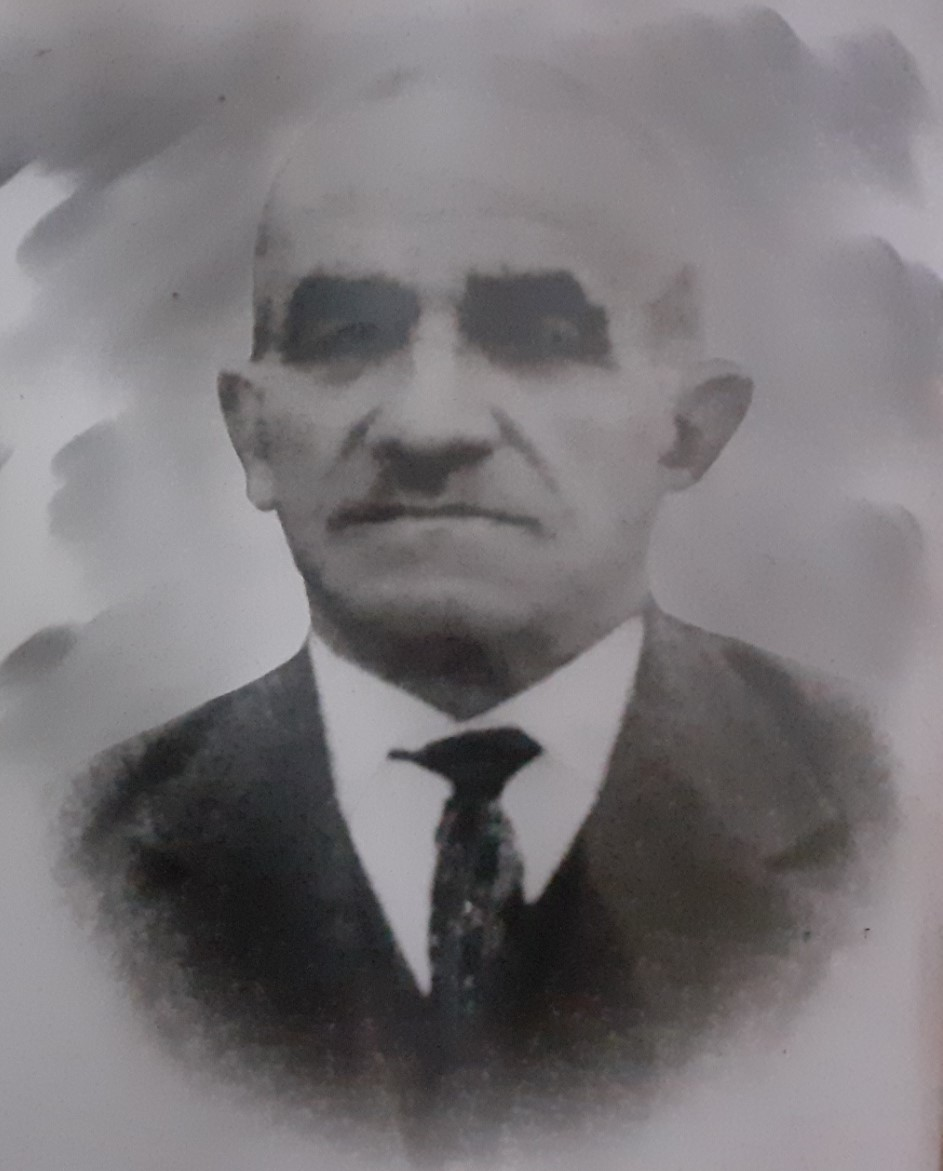
\includegraphics[width=\linewidth]{p1-Adelino.jpg}
			\caption{ p1-Adelino }
		\end{minipage}
		\hspace{1cm} % add some horizontal space here
		\begin{minipage}{0.3\textwidth}
			\begin{tcolorbox}[colback=white, colframe=black, boxrule=1pt]
				\begin{itemize}
					\item jpg
                    
				\end{itemize}

			\end{tcolorbox}
		\end{minipage}
	\end{figure}
	
\clearpage




	\section{Meta-information}
	\newcounter{tablecounter2}

	
		\stepcounter{tablecounter2}
		\begin{table}[ht!]
			\centering
			\begin{tabular}{|c|c|}
				\hline
				
					\textbf{ id } & \textit{ IndustriasReunidasvilar } \\
					\hline
				
					\textbf{ format } & \textit{ latex } \\
					\hline
				
					\textbf{ type } & \textit{ Story } \\
					\hline
				
					\textbf{ date } & \textit{ 1957 } \\
					\hline
				
			\end{tabular}
			\caption{A \textbf{ Story }-\textit{ IndustriasReunidasvilar }} % Add a caption to the table with the current table counter value
			\label{table:\arabic{tablecounter2}} % Use the current table counter value as the label name
		\end{table}
	
		\stepcounter{tablecounter2}
		\begin{table}[ht!]
			\centering
			\begin{tabular}{|c|c|}
				\hline
				
					\textbf{ id } & \textit{ EducaçãoPrimária } \\
					\hline
				
					\textbf{ format } & \textit{ latex } \\
					\hline
				
					\textbf{ type } & \textit{ Story } \\
					\hline
				
					\textbf{ date } & \textit{ 2022 } \\
					\hline
				
			\end{tabular}
			\caption{A \textbf{ Story }-\textit{ EducaçãoPrimária }} % Add a caption to the table with the current table counter value
			\label{table:\arabic{tablecounter2}} % Use the current table counter value as the label name
		\end{table}
	

\clearpage

\section{Time Frame}

\newcommand{\foo}{\hspace{-2.3pt}$\bullet$ \hspace{5pt}}

\scalebox{1}{
\begin{tabular}{r |@{\foo} l}

\end{tabular}
}


\end{document}